\documentclass{article}
\usepackage{graphicx}         % For inserting images
\usepackage{amsmath, amsfonts, amsthm}  % AMS packages for math
\usepackage{float}            % For improved figure placement
\usepackage{geometry}         % To customize page dimensions
\geometry{margin=1.25in}
\usepackage{csquotes}         % Context sensitive quotes
\usepackage{url}              % URL formatting
\usepackage{forest}           % For drawing trees
\usepackage{hyperref}         % For hyperlinks
\usepackage{tikz}             % For drawing diagrams
\usepackage{algorithm}        % For pseudocode algorithms
\usepackage{algpseudocode}    % For pseudocode
\usetikzlibrary{quantikz2}    % For Quantum circuit diagrams
\setlength{\parindent}{0cm}
\addtolength{\oddsidemargin}{-2cm}
\addtolength{\evensidemargin}{-2cm}
\setlength{\textwidth}{18cm}
\addtolength{\topmargin}{-2cm}
\setlength{\textheight}{24cm}
\addtolength{\parskip}{5mm}

\title{IFT6135 -- Apprentissage de Représentations (Deep Learning)}
\author{F. Wilhelmy \\
    \texttt{fwilhelmy@hotmail.com}}
\date{Automne 2024}

\begin{document}

\maketitle

% Title page (centered)
\begin{center}
    \huge IFT6135-H25 \\
    \Large Notes du cours -- Hivers 2022 \\
    \vspace{1cm}
    Montreal, QC \\
    \vspace{1cm}
\end{center}
\newpage
\section*{Introduction}
These are my personal notes from the course IFT6135 — Representation Learning — taught by Aaron Courville at MILA in Montreal, Quebec, during the Winter 2025 semester. The course ran from January to April, and it was a deep (pun intended) dive into the theory and practice of learning useful representations from data.

That said — fair warning! These notes are incomplete, sometimes messy (I often switch between French and English), and occasionally wrong. They reflect my own understanding of the material, and I’ve tried my best to make sense of complex ideas. Some parts were generated or cleaned up with the help of ChatGPT, others go slightly beyond what was taught in class. There are definitely missing citations, and I still plan to add more figures and references.

I’m sharing these in case they help others going through this intense (but rewarding!) course. If you spot errors, have suggestions, or want to expand a section, feel free to fork the repo and open a pull request. I’ll do my best to review changes promptly. If you do contribute, please don’t forget to add your name to the author list!

A sincere thank you to Professor Aaron Courville for his inspiring lectures, to the TAs for crafting such challenging and thought-provoking assignments, and to all the students — especially Thomas, Maël and Olivier — whose discussions, questions, and collaboration made the learning process far more engaging. It was a real privilege to be part of such a passionate and driven group.

And for those reading this outside the context of MILA — welcome! You’ll probably get the most out of these notes if you already have some background in math, computer science, and deep learning. A solid starting point is the Deep Learning book: \url{https://www.deeplearningbook.org/}.

Enjoy the ride — and good luck with your learning journey!

\newpage

\tableofcontents
\newpage

\section{History} \label{sec:history}

\begin{figure}[ht]
    \centering
    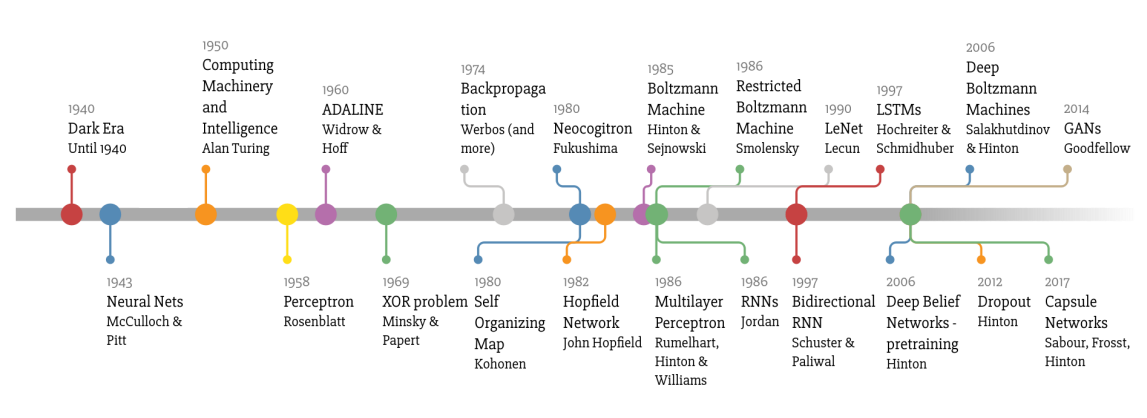
\includegraphics[width=1\linewidth]{graphics/ai_history.png}
    \caption{Contexte historique}
    \label{fig:ai-history}
\end{figure}

\paragraph{Naissance de l'IA (années 1950)}
Le début du domaine de l'IA (intelligence artificielle) a eu lieu vers 1950.
\begin{itemize}
    \item Perceptron de McCulloch et Pitts (modèle de neurone artificiel).
    \item Apprentissage de Rosenblatt (introduction du calcul de l'erreur).
    \item Théorie du calcul de Turing.
    \item Théorie de l'information de Shannon.
\end{itemize}

Le neurone artificiel est une inspiration de son homologue biologique. Il est composé d'entrées, de poids et d'une fonction d'activation. Initialement, il n'existait pas de mécanisme d'apprentissage. Rosenblatt a introduit un apprentissage basé sur le calcul de l'erreur, mais sans descente de gradient, limitant les réseaux à une seule couche.

\paragraph{Premier hiver de l'IA (années 1960-1970)}
Le problème du XOR soulevé par Minsky et Papert a mis en évidence une limitation majeure du perceptron, menant à un désintérêt général pour l'IA et à une réduction des investissements dans le domaine. C'est à cette époque que les Multi-Layer Perceptrons (MLP) ont été introduits, permettant de dépasser la contrainte de séparabilité linéaire des données. L'introduction de la \textbf{rétropropagation} a marqué une avancée majeure :
\begin{itemize}
    \item \textbf{Efficace} : Complexité de \( O(N) \), où \( N \) est le nombre d'exemples.
    \item \textbf{Générique} : Basé sur la descente de gradient, encore utilisé aujourd'hui.
    \item \textbf{Local} : Aucune garantie de trouver une solution optimale globale.
\end{itemize}

\paragraph{Retour de l'IA (années 1990)}
Dans les années 1990, l'intelligence artificielle a connu un renouveau avec l'apparition de nouveaux modèles :
\begin{itemize}
    \item \textbf{LeNet} de Yann LeCun, utilisé pour la reconnaissance automatique de caractères.
    \item \textbf{Réseaux récurrents} développés par Hochreiter et Schmidhuber, permettant la représentation de séquences.
\end{itemize}

\paragraph{Deuxième hiver de l'IA (années 2000)}
Un nouvel hiver de l'IA est survenu, causé principalement par :
\begin{itemize}
    \item Le problème du \textit{vanishing gradient}, empêchant l'entraînement des réseaux de plus de 3-4 couches.
    \item Le manque de justification théorique des performances des réseaux de neurones.
    \item L'apparition des SVMs (machines à vecteurs de support) qui offraient des performances comparables avec moins de complexité et d'hyper-paramètres.
\end{itemize}

\paragraph{Début de l'apprentissage profond (2006)}
À partir de 2006, des méthodes ont été développées pour entraîner efficacement des réseaux de neurones profonds :
\begin{itemize}
    \item Deep Boltzmann Machines.
    \item Deep Belief Networks.
    \item Pré-entraînement non supervisé et apprentissage par couche.
\end{itemize}
L'entraînement des autoencodeurs par couche était alors fastidieux, nécessitant des sous-entraînements successifs.

\paragraph{Explosion de l'apprentissage profond (2012-2013)}
L'année 2012 marque un tournant majeur avec l'introduction d'AlexNet (SuperVision) lors de la compétition ImageNet. Plusieurs innovations ont contribué à ce succès :
\begin{itemize}
    \item Fonction d'activation \textbf{ReLU}.
    \item \textbf{Augmentation des données} pour améliorer la robustesse des modèles.
    \item \textbf{Réseaux convolutifs} pour extraire des caractéristiques hiérarchiques des images.
    \item \textbf{Utilisation des GPUs}, rendant l'entraînement des modèles plus rapide et efficace.
    \item Accès à de grandes bases de données comme ImageNet.
\end{itemize}

\subsection*{Aujourd'hui}
L'apprentissage profond est omniprésent et trouve des applications variées dans de nombreux domaines.

% =============================================================
\clearpage\newpage

\section{Fundamental Concepts}

\subsection{Définition de l’apprentissage machine}
La programmation 'manuelle' est un processus/algorithme qui a comme entrée des données et des instructions (règles) et qui produit une sortie.

À l'inverse, l'apprentissage machine est un système où l'on fournit en entrée des données et la réponse attendue pour une certaine donnée. La sortie de ce système est un ensemble de règles (modèle) qui cherche à généraliser une relation entre les données et leur sortie respective.

\begin{figure}[ht]
    \centering
    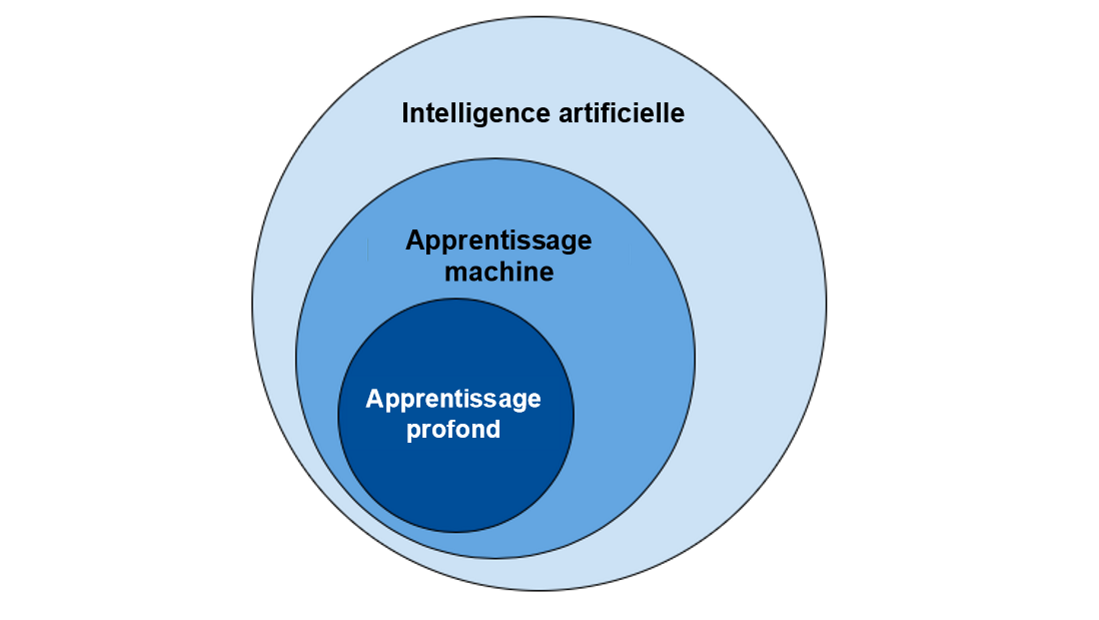
\includegraphics[width=0.5\linewidth]{graphics/ai_terms.PNG}
    \caption{Terminologie de l'IA}
    \label{fig:ai-terms}
\end{figure}

\begin{figure}[ht]
    \centering
    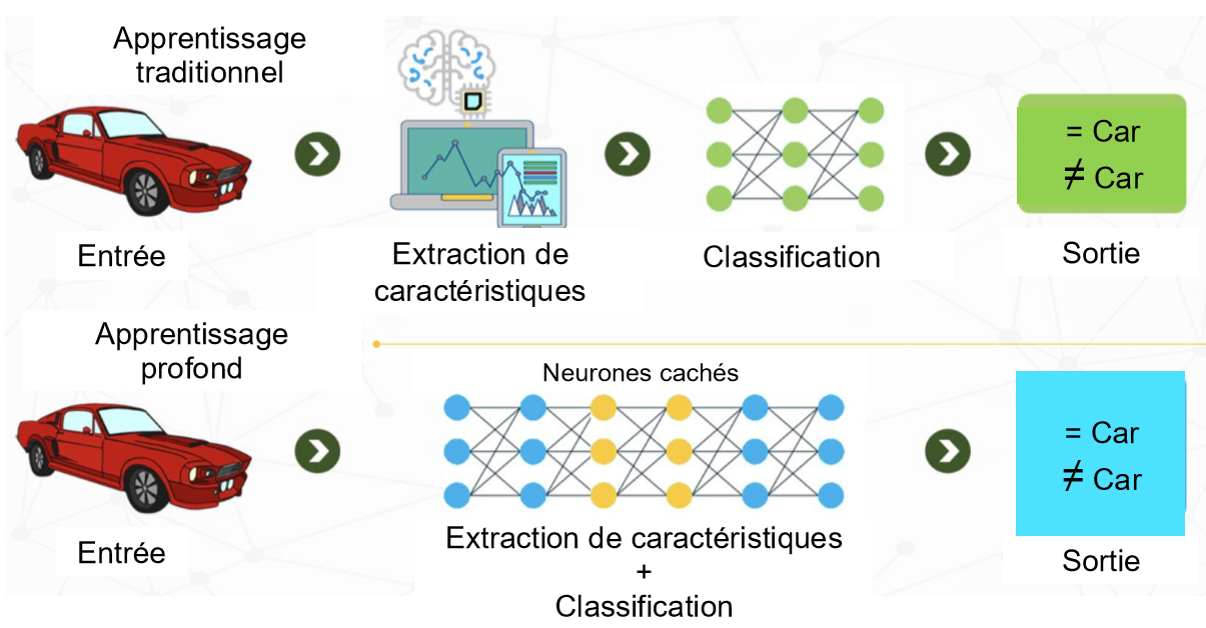
\includegraphics[width=0.7\linewidth]{graphics/ml_vs_dl.PNG}
    \caption{Différence entre l'apprentissage machine et l'apprentissage profond}
    \label{fig:ai-terms-dl}
\end{figure}

\subsection{Le Perceptron}
Le perceptron est le bloc de construction de base dans les réseaux de neurones. Deux composants essentiels :
\begin{enumerate}
    \item \textbf{La somme pondérée (\(net_j\)) :}
    \[
    net_j = \sum_{i=0}^{n} x_i w_{ij} = \vec{w}_j \cdot \vec{x} = \mathbf{w}_j \mathbf{x}
    \]
    ou, en termes du produit scalaire et de l’angle \(\alpha\),
    \[
    net_j = |\mathbf{w}_j| |\mathbf{x}| \cos(\alpha).
    \]
    
    \item \textbf{La fonction d'activation (\(F\)) :} introduit la non-linéarité en activant ou désactivant le neurone selon l’agrégation pondérée des entrées.
\end{enumerate}

\begin{figure}[H]
    \centering
    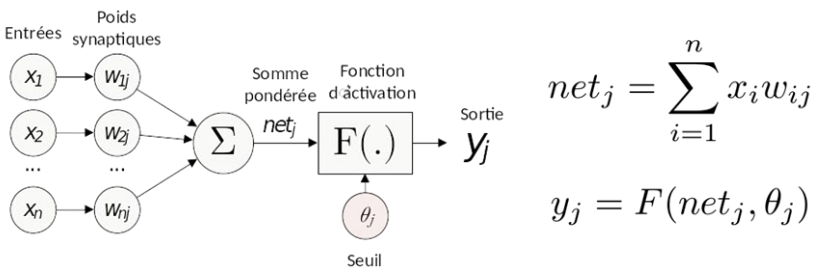
\includegraphics[width=\linewidth]{graphics/perceptron.png}
    \caption{Schéma d’un perceptron}
    \label{fig:perceptron}
\end{figure}

Note importante : Une caractéristique importante du perceptron est qu'il est sensible à l'ordre des données d'entrée. Deux ensembles de données identiques mais présentés dans un ordre différent peuvent produire des ajustements de poids différents.

L'ajustement des poids par la correction de l'erreur a permis au perceptron d'apprendre, mais il n'était pas capable de résoudre certains problèmes comme le problème du XOR. Cette limitation a été surmontée avec l'introduction de méthodes d'optimisation plus avancées, telles que la descente de gradient. Cependant, le choix de la fonction d'activation dans ces méthodes est crucial pour assurer un apprentissage efficace.

\subsection{Neural Networks Layer (NEW)}
In a deep neural network, we can find multiple layers of different functions. The most basic one is a Fully Connected Layer.

For an input of \(N_{in}\) neurons and an output of \(N_{out}\) neurons:
\[
\text{Total Parameters} = N_{in} \times N_{out} + N_{out}.
\]

\subsection{Conception d’un Modèle}
La conception d'un modele d'apprentissage profond peut être décomposée en 4 étapes :
\begin{itemize}
	\item Definition de la taches et du dataset
    \item \textbf{Sélection du modèle}
    \item \textbf{Choix de la fonction de coût}
	\item Optimisation du modele
\end{itemize}

\subsubsection{Le Modèle}
Un modèle efficace doit généraliser et représenter les données. Le choix dépend aussi des contraintes de déploiement (puissance de calcul, rapidité, etc.) et il peut être pertinent de se demander si l'utilisation de l'IA est nécessaire ou si un algorithme plus simple pourrait suffire.

\subsubsection{L’Optimisation}
Cette phase cherche la configuration optimale des paramètres dans l’espace de la fonction de coût. La validation permet d’éviter les problèmes de surapprentissage et de sous-apprentissage.

\begin{figure}[ht]
    \centering
    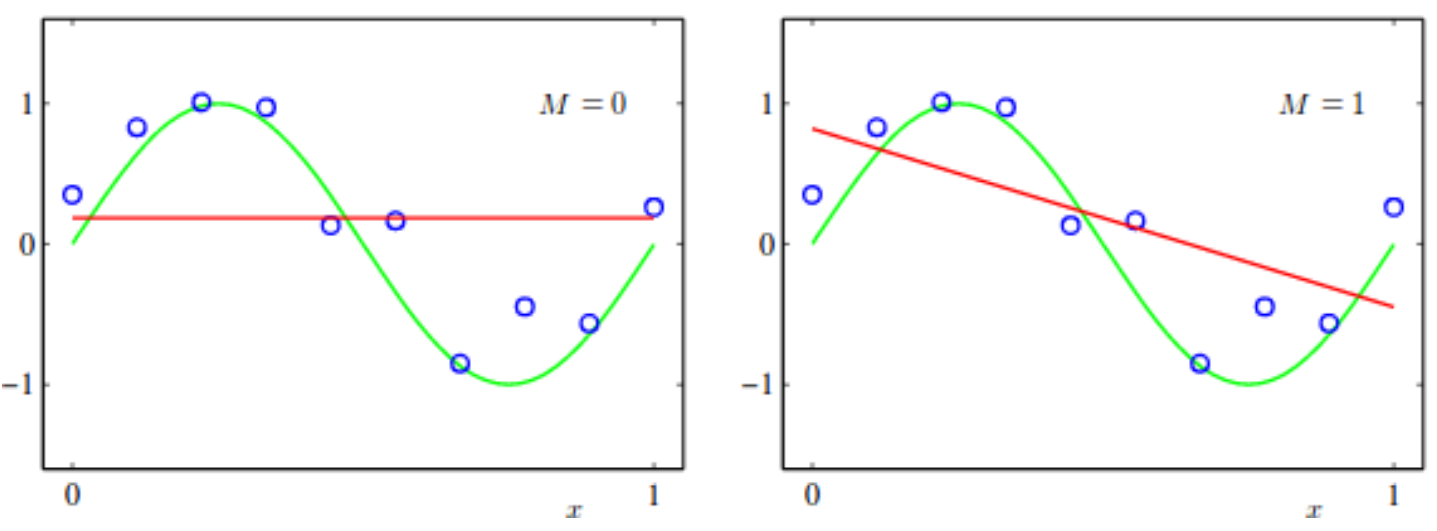
\includegraphics[width=\linewidth]{graphics/sous-apprentissage.PNG}
    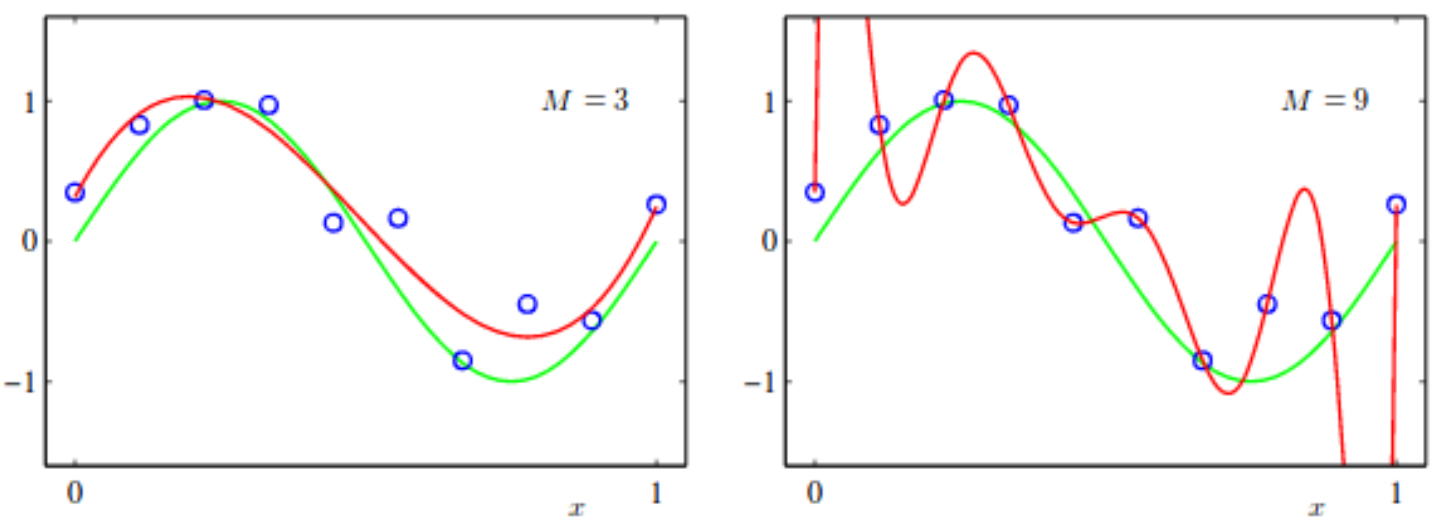
\includegraphics[width=\linewidth]{graphics/sur-apprentissage.PNG}
    \caption{Exemple de surapprentissage (overfit) et de sous-apprentissage (underfit)}
    \label{fig:over-under-fit}
\end{figure}

\subsection{Types de Problèmes}

\begin{itemize}
    \item \textbf{Régression :} \(x \xrightarrow{} \mathbb{R}\)
    \item \textbf{Classification :} \(x \xrightarrow{} \mathbb{N}\)
\end{itemize}

\subsection{Types de Modèles}
Les approches de l'apprentissage machine se classent en différentes familles :
\begin{itemize}
    \item \textbf{Supervisé :} Toutes les données sont étiquetées.
    \item \textbf{Non-supervisé :} Aucune étiquette n’est disponible.
    \item \textbf{Semi-supervisé :} Seule une partie des données est étiquetée.
    \item \textbf{Auto-supervisé :} Des étiquettes peu coûteuses sont générées pour des tâches auxiliaires.
    \item \textbf{Apprentissage par renforcement :}
\end{itemize}

\begin{figure}[ht]
    \centering
    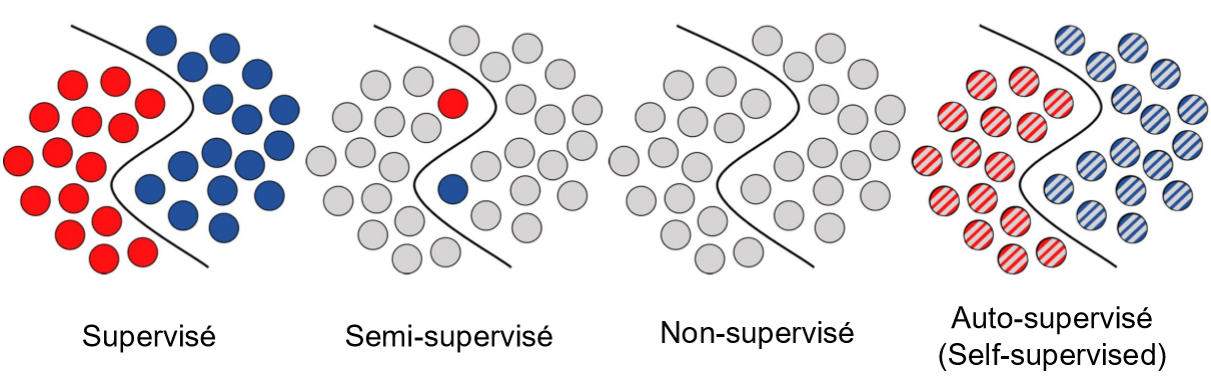
\includegraphics[width=\linewidth]{graphics/learning_type.png}
    \caption{Différents types d’apprentissage}
    \label{fig:learning-types}
\end{figure}

\subsection{Inductive Bias in Machine Learning}
Inductive bias refers to the assumptions a model makes to generalize from training data to unseen data. Different architectures (e.g., CNNs, RNNs, Transformers) incorporate unique biases that affect how they learn and represent information.

Given that real-world data is limited, an inductive bias enables a model to make reasonable predictions by imposing constraints on the possible functions it can learn.

Deep learning architectures have specific biases that give them particular strengths and limitations. For instance, CNNs exploit spatial locality, while Transformers capture long-range dependencies using attention mechanisms.

\begin{itemize}
    \item \textbf{Smoothness Bias}: Similar inputs yield similar outputs.
    \item \textbf{Linear Separability}: Data can be separated by a linear boundary (used in logistic regression and SVMs).
    \item \textbf{Locality Bias}: Local structures are emphasized (as in CNNs).
    \item \textbf{Sequential Dependence}: Past information influences future predictions (as in RNNs).
    \item \textbf{Attention-Based Bias}: Certain input features are weighted more heavily (as in Transformers).
	\item \textbf{Manifold Hypothesis}:
\end{itemize}

Depending on the level of bias imposed on the modele, we get different results.

\begin{itemize}
    \item \textbf{Strong Inductive Bias:} Imposes strong assumptions for faster learning but reduced flexibility (e.g., linear regression).
    \item \textbf{Weak Inductive Bias:} Fewer assumptions allow greater flexibility but require more data (e.g., deep neural networks).
\end{itemize}

\subsection{Bias-Variance Tradeoff}
The overall error can be decomposed as:
\[
\text{Total Error} = \text{Bias}^2 + \text{Variance} + \sigma^2,
\]
with
\[
\text{Bias}[\tilde{f}] = E[\tilde{f}] - f \quad \text{and} \quad \text{Variance}[\tilde{f}] = E\big[(\tilde{f} - E[\tilde{f}])^2\big].
\]

\begin{figure}[ht]
    \centering
    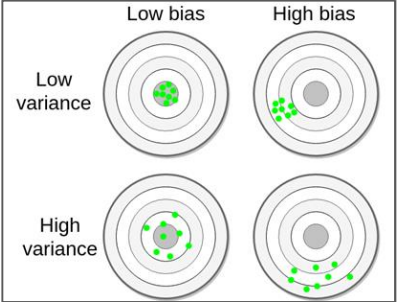
\includegraphics[width=\linewidth]{graphics/biais-variance.png}
    \caption{Bias versus Variance}
    \label{fig:biais-variance}
\end{figure}

% =============================================================
\clearpage\newpage

\section{Optimization Methods} \label{sec:optimization}
Optimization methods search for the best parameter configuration by minimizing the loss function. Generally, optimization techniques will focus on improving the training accuracy of the model and tit's convergeance speed. Asopposed to regularisation techniques (that we will cover lated that are more focused on the ability of the model to generlise . Therefor soetimes slwolying the training. En d'autre mot, elle va determiné si on réussis a trouvé le minimum de notre fonction de cout (loss function).

\begin{itemize}
    \item Evolutionary algorithms.
    \item Closed-form solutions.
    \item Gradient-based methods (first and second order).
\end{itemize}

In this section, we will mostly focus on first-order gradient-based methods.

\subsection{Optimizers}
\subsubsection{Stochastic Gradient Descent (SGD)}
SGD updates parameters using mini-batches:
\begin{algorithm}[H]
\caption{Stochastic Gradient Descent}
\begin{algorithmic}[1]
    \State \textbf{Input:} Learning rate \(\eta\), initial parameter \(\theta\)
    \While{Stopping criterion not met}
        \State Sample a mini-batch of \(m\) examples \((x^{(i)}, y^{(i)})\)
        \State Compute gradient estimate:
        \[
        \hat{g} = \frac{1}{m} \sum_{i=1}^{m} \nabla_\theta L(f(x^{(i)}; \theta), y^{(i)})
        \]
        \State Update parameters:
        \[
        \theta \leftarrow \theta - \eta \hat{g}
        \]
    \EndWhile
\end{algorithmic}
\end{algorithm}

\subsubsection{Momentum}
Le \textbf{gradient avec moment} est une méthode d'optimisation qui améliore la convergence des algorithmes de descente de gradient en ajoutant une notion d'accumulation des gradients passés. Cela aide à surmonter les oscillations et à accélérer la convergence dans des directions où le gradient varie peu. Cette méthode peut aussi être combinée avec d'autres techniques d'optimisation, comme le redémarrage à chaud et l'ajustement adaptatif du taux d'apprentissage.
\begin{figure}[h]
    \centering
    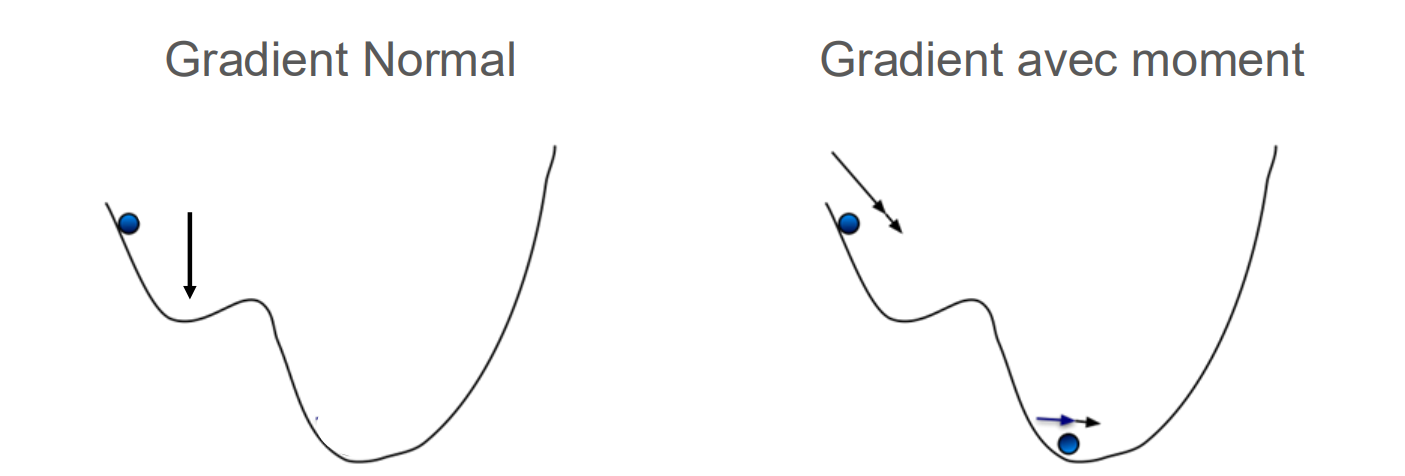
\includegraphics[width=1 \linewidth]{graphics/gradient_with_moment.PNG}
    \caption{Gradient avec moment}
    \label{fig:gradient_with_moment}
\end{figure}

La mise à jour des poids en utilisant le gradient avec moment se fait selon la règle suivante :
\[
v_{t+1} = \rho v_t - \eta \nabla L(f(x;\theta_t), y)
\]
\[
\theta^{t+1} = \theta^t + v_{t+1}
\]
where \(\rho\) is the momentum coefficient.

\subsubsection{Nesterov Accelerated Gradient (NAG)}
Une variante du gradient avec moment est le \textbf{moment de Nesterov}, qui prévoit le déplacement avant de calculer le gradient. Cette approche permet d'anticiper le comportement de la fonction de perte et d'améliorer encore davantage la convergence. Elle aide à réduire les oscillations et à améliorer la vitesse d'apprentissage dans des zones planes de l'espace des solutions.

Nesterov Momentum refines the momentum method by first applying a partial update before computing the gradient, allowing for more accurate gradient adjustments.
\[
\tilde{\theta} = \theta + \alpha v,
\]
\[
g = \nabla_\theta L(\tilde{\theta}),
\]
\[
v \leftarrow \alpha v - \eta g,\quad \theta \leftarrow \theta + v.
\]

\subsubsection{ADAGRAD (Adaptive Gradient)}
Adagrad adapts the learning rate for each parameter for each parameter using accumulated squared gradients, making it suitable for convex problems but potentially slowing down over time due to accumulated gradients.
\[
r \leftarrow r + g \odot g,
\]
Here $r$ accumulates past squared gradients element-wise.
\[
\Delta \theta = \frac{\eta}{\sqrt{r} + \epsilon} \odot g,
\]
Here $\epsilon$ is a small constant for numerical stability.
\[
\theta \leftarrow \theta - \Delta \theta.
\]
\subsubsection{RMSPROP}

TODO 

\subsubsection{ADAM (Adaptive Moment Estimation)}
This optimiser combines RMSPROP and momentum, computing adaptive learning rates for each parameter by using both first-order moment estimates (momentum) and second-order moment estimates (variance).

We compute the first moment estimate $m$ (moving average of gradients) and the second moment estimate $v$ (moving average of squared gradients) as 
\[
m \leftarrow \beta_1 m + (1 - \beta_1) g,\quad v \leftarrow \beta_2 v + (1 - \beta_2) g \odot g,
\]
Where $\beta_*$ is is the decay rate.
\[
\hat{m} = \frac{m}{1 - \beta_1^t},\quad \hat{v} = \frac{v}{1 - \beta_2^t},
\]

The bias correction terms $\hat{m}$ and $\hat{v}$ are then used to  adjust for the initialization bias.
\[
\Delta \theta = \frac{\eta}{\sqrt{\hat{v}} + \epsilon} \odot \hat{m},\quad \theta \leftarrow \theta - \Delta \theta.
\]

Adam is widely used due to its robustness and ability to handle sparse gradients.

\subsubsection{ADAMW}
The succesor of ADAM, who is also very popular. This method decouples weight decay from gradient updates, improving generalization.
% TODO add more details

\subsubsection{AMSGRAD}
This optimiser ensures non-increasing second moment estimates to address convergence issues in ADAM.
%TODO add more details

\subsubsection{ADABOUND}
This optimiser dynamically bounds the learning rate to transition smoothly between adaptive methods and SGD.
%TODO add more details

\subsection{Normalization} (NEW)
Normalization accelerates training and stabilizes gradient flow by standardizing activations.

\begin{figure}
    \centering
    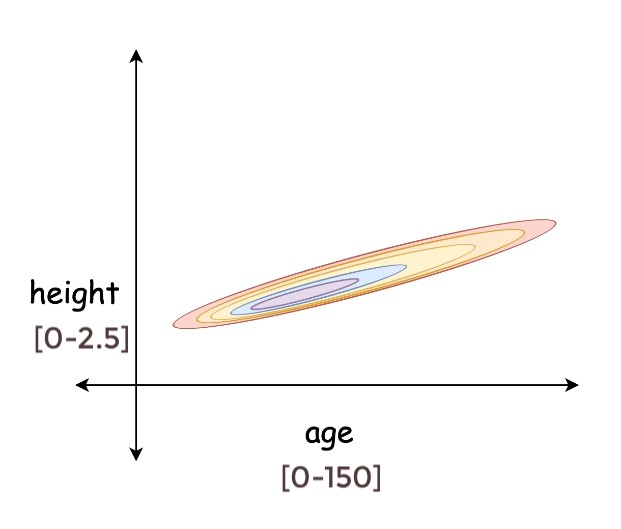
\includegraphics[width=0.4\linewidth]{graphics/batchnorm_exp01.jpg}
    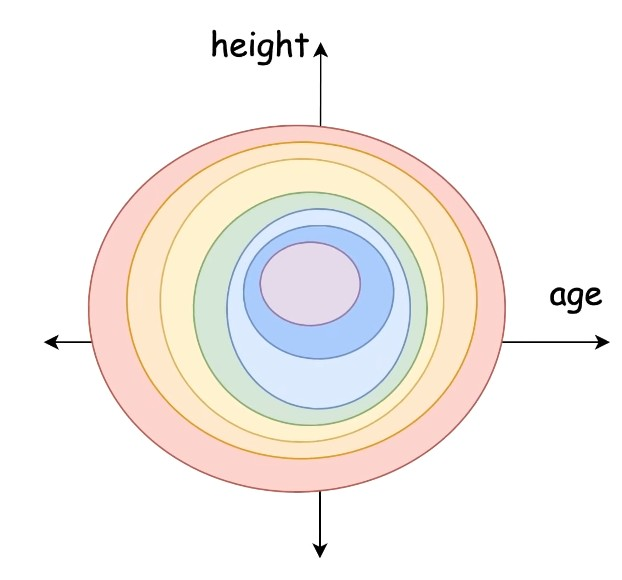
\includegraphics[width=0.4\linewidth]{graphics/batchnorm_exp02.jpg}
    \caption{Gradient landscape without and with normalization}
    \label{fig:enter-label}
\end{figure}

Normalizing inputs (or activations) helps reduce the impact of differing value ranges, smoothing the loss landscape and improving gradient flow.

As we can see in figure \ref{fig:enter-label}, the landscape of normalized data will be much easier to traverse during training. Without it, there are some locations that could be complicated to get out of and some points are much further away than others. In the normalized case, everything is "relatively" close.

This will also make initialization less critical and leads to faster convergence from various starting points.

Once the parameters are normalised, the learned parameters \(\gamma\) and \(\beta\) are applied:
\[
\hat{x}_i = \frac{x_i - \mu}{\sqrt{\sigma^2 + \epsilon}},\quad y_i = \gamma \hat{x}_i + \beta.
\]

In neural networks, we can apply layers of normalisation to the data. In such a layer, for \(D\) features, there are \(2 \times D\) trainable parameters (\(\gamma\) and \(\beta\)).
\textbf{Parameters:}
\[
\text{Total Parameters} = 2 \times D,
\]
accounting for $\gamma$ and $\beta$ per feature (aside from non-trainable running statistics).

\subsubsection{Batch Normalization}
\label{sec:batchnorm}

\textbf{Reference:} Ioffe, Szegedy (ICML 2015)

Batch Normalization (BN) normalizes activations across each channel for all samples in a batch.  
Given batch of examples of size $B$, with channels $C$ and features $F$, we compute:
\[
\mu_c = \frac{1}{B*F} \sum_{B,F} x_{bcf}, 
\quad
\sigma^2_c = \frac{1}{B*F} \sum_{B,F} (x_{bcf} - \mu_c)^2.
\]

\begin{itemize}
    \item Works well in image processing. Typically inserted between linear/convolution layers and the nonlinearity.
    \item Works well for large mini-batch sizes.
\end{itemize}

\subsubsection{Layer Normalization}
\label{sec:layernorm}

\textbf{Reference:} Ba, Kiros, Hinton

Layer Normalization (LN) normalizes across the features (hidden units) within a single layer for each sample. Given batch of examples of size $B$, with channels $C$ and features $F$, we compute:
\[
\mu_b = \frac{1}{C*F} \sum_{C,F} x_{bcf}, 
\quad
\sigma^2_b = \frac{1}{C*F} \sum_{C,F} (x_{bcf} - \mu_b)^2.
\]

\begin{itemize}
    \item Often used in RNNs and Transformers (especially when mini-batches are small or variable in size).
    \item Normalization is independent for each training example.
\end{itemize}

\subsubsection{Instance Normalization}
\label{sec:instancenorm}

Instance Normalization (IN) normalizes across spatial dimensions for each channel and for each sample independently. It is frequently used in style transfer tasks. Given batch of examples of size $B$, with channels $C$ and features $F$, we compute:

\[
\mu_{bc} = \frac{1}{F} \sum_{F} x_{bcf}, 
\quad
\sigma^2_{bc} = \frac{1}{F} \sum_{F} (x_{bcf} - \mu_{bc})^2.
\]

\begin{itemize}
    \item Each sample-channel is normalized independently.
    \item Helps in style transfer by normalizing per-image and per-channel statistics.
\end{itemize}

\subsubsection{RMS Normalization}
\label{sec:rmsnorm}

RMS Normalization (RMSNorm) is similar to LayerNorm but normalizes based on the root mean square of the features rather than the variance:
\[
\mu_{\text{b}}^2 = \frac{1}{C*F} \sum_{C,F} x_{bcf}^2
\quad\text{and}\quad
\hat{x}_{bcf} = \frac{x_{bcf}}{\sqrt{\mu_b^2 + \epsilon}}
\]

\begin{itemize}
    \item Does not subtract a mean; only divides by the root mean square.
    \item Useful in large-scale models due to reduced computational cost compared to LayerNorm.
\end{itemize}

\subsubsection{Group Normalization}
\label{sec:groupnorm}

\textbf{Reference:} Wu and He (2018)

Group Normalization (GN) normalizes by splitting channels into $G$ groups, then normalizing each group’s mean and variance.

\begin{itemize}
    \item Bridges the gap between LayerNorm and InstanceNorm.
    \item Works well when mini-batch sizes are small.
\end{itemize}

\subsubsection{Weight Normalization}
\label{sec:weightnorm}

Weight Normalization (WN) normalizes the weights (rather than activations). It reparameterizes a weight vector $\mathbf{w}$ as
\[
\mathbf{w} = \frac{g}{\|\mathbf{v}\|} \mathbf{v},
\]
where $\mathbf{v}$ is a learned direction and $g$ is a learned scalar. Then the output is:
\[
y = \phi(\mathbf{w} \cdot \mathbf{x} + b).
\]
\begin{itemize}
    \item Decouples the magnitude of the weights from their direction.
    \item Simplifies optimization by controlling the length of the weight vector explicitly.
\end{itemize}

% =============================================================
\clearpage\newpage

\section{Regularization} \label{sec:regularization}
A central problem in machine learning is how to make an algorithm that will perform well not just on the training data, but also on new inputs. Many strategies used in machine learning are explicitly designed to reduce the test error, possibly at the expense of increased training error. These strategies are known collectivelyas regularization. A great many forms of regularization are available to the deep learning practitioner.

\subsection{L2 Regularization}
TODO..
% TODO: Add more details on L2 regularization.

\subsection{L1 Regularization}
TODO..
% TODO: Add more details on L1 regularization.

\subsection{Early Stopping}
This algorithm allows us to stop the training when we see the performance on the validation set reducing.

\subsubsection{Variants}
There exist techniques that are not very used recently but are still worth mentioning such as

\begin{itemize}
\item \textbf{Early Stopping with Retraining:} This technique is made to not waste certain example in the validation set and uses validated examples for a minor performance boost. It's not very popular because it's not the goal to grab this little performance gain and the data base are very big now.
\item \textbf{Early Stopping with Surrogate Loss:} Employs an alternate loss function.
\end{itemize}

\subsection{Dropout Training}
Randomly disables certain connections during training to reduce overfitting.
%TODO add more details 

\subsection{Stochastic Depth}
Randomly drop entire layers during training, particularly effective in ResNets.

\subsection{Transfer Learning}
Train a general model and fine-tune it for specific tasks.

\subsection{Multi-Task Learning}
Build a general model and plug in smaller task-specific modules.
\begin{figure}[ht]
    \centering
    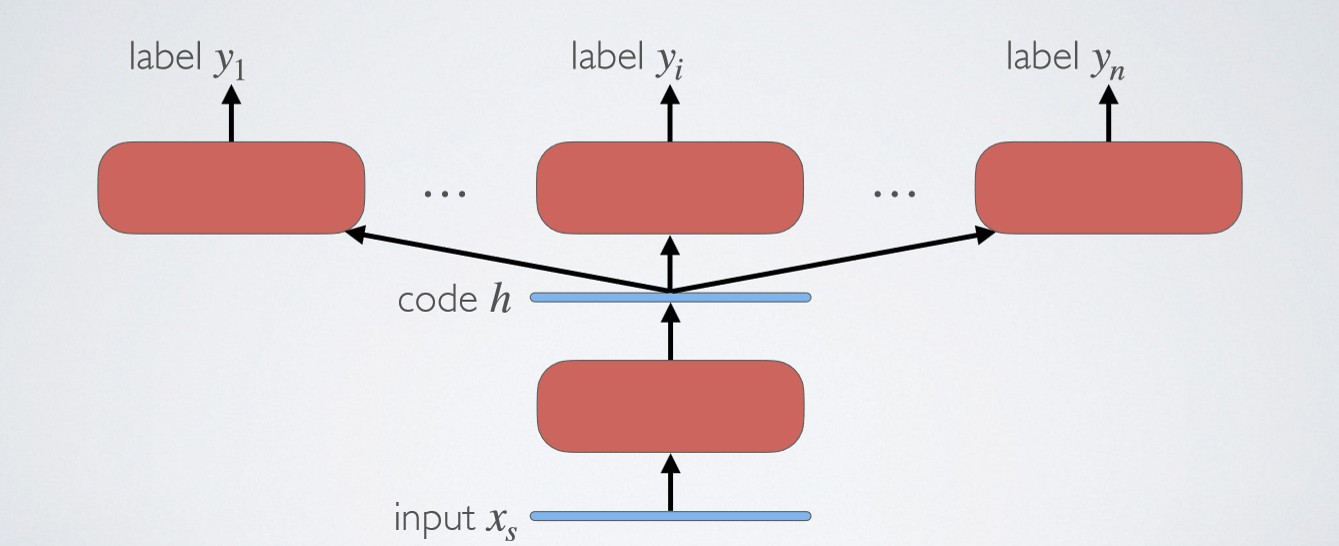
\includegraphics[width=\linewidth]{graphics/multitask-learning.jpg}
    \caption{Multi-Task Learning architecture}
    \label{fig:multitask-learning}
\end{figure}

\subsection{Label Smoothing}
Replace hard labels (0 and 1) with smoothed values to improve generalization. This results in a cluster of labels together.
% TODO: Add precise equations.

\begin{figure}
    \centering
    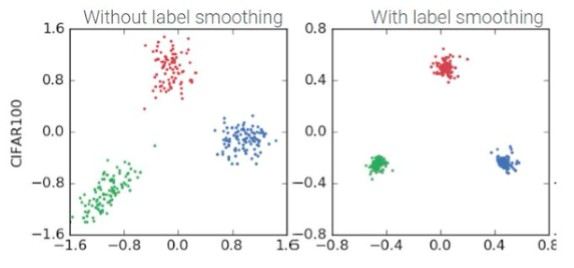
\includegraphics[width=1\linewidth]{graphics/label-smoothing.jpg}
    \caption{Source: When does label smoothing help?}
    \label{fig:enter-label}
\end{figure}

\subsection{Data Augmentation}
Increase dataset size by applying transformations (translation, rotation, etc.). This technique had a HUGE impact on the image, audio, video and other tasks with those type of data but NONE to others like text because there is no way found so far to augment text.

\subsubsection{Data Augmentation for Images}
% TODO add visualisation of the techniques

\paragraph{RandAugment} This technique is among the most popular. In general, it applies transformations such as: translation, rotation, scaling, equalization, posterization and solarization, etc...

However, more aggressive augmentation techniques exist..

\paragraph{MixUp} Blends two images and their labels. This technique generally yields low performance.

\paragraph{Random Erasing / Cutout} Removes a random portion of the image.

\paragraph{CutMix} Combines regions from different images with proportional labels.

% =============================================================
\clearpage\newpage

\section{Convolutional Neural Networks (CNNs)} \label{sec:cnn}
A Convolutional Neural Network (CNN) is a type of neural network designed specifically for pattern recognition in image or audio data (mimicking the way the visual cortex processes visual information). CNNs leverage convolution operations to extract hierarchical features from images, efficiently handling high-dimensional data while exploiting spatial structures, such as the relationship between nearby pixels. This architecture builds invariance to transformations like translation, making it highly effective for image-related tasks. A typical CNN consists of alternating convolutional and pooling layers, followed by fully connected layers.

\subsection{Key Features}
\paragraph{Local Connectivity} Each neuron connects only to a local region of the input, called the \textit{receptive field}. This allows CNNs to focus on localized patterns (e.g., edges, textures), reducing the number of parameters compared to fully connected networks (FFNs).

\paragraph{Parameter Sharing} The same set of weights (kernel) is used across different spatial locations of the input, significantly reducing computational complexity.
\paragraph{Pooling (Dimensionality Reduction)} Reduces the number of hidden units in the model and helps achieve translational invariance, improving generalization.

For an image \(x\), a kernel \(k\), and output \(y\):
\[
(y * k)_{i,j} = \sum_{p,q} x_{i+p,j+q} \cdot k_{r-p, r-q}.
\]

\subsection{Convolution Layer}
For an input of size \(N \times N \times D_{in}\), kernel of size \(K \times K\), stride \(S\), padding \(P\), and \(D_{out}\) filters:
\[
N_{out} = \left\lfloor \frac{N - K + 2P}{S} \right\rfloor + 1,
\]
with total parameters:
\[
\text{Total Parameters} = D_{out} \times \left( K \times K \times D_{in} + \text{(bias term)} \right).
\]

\subsection{Pooling Layer}
For input of size \(N \times N \times D\), pooling window \(F \times F\), and stride \(S\):
\[
N_{out} = \left\lfloor \frac{N - F}{S} \right\rfloor + 1,
\]
with zero trainable parameters. There are two main types of pooling

\begin{itemize}
    \item \textbf{Max Pooling:}
    \[
    y_{i,j} = \max_{(p,q) \in R} x_{i+p, j+q}.
    \]
    \item \textbf{Average Pooling:}
    \[
    y_{i,j} = \frac{1}{|R|} \sum_{(p,q) \in R} x_{i+p, j+q}.
    \]
\end{itemize}

% TODO adding something from this might be interesting : https://guandi1995.github.io/Pooling-Layers/#:~:text=In%20summary%2C%20since%20there%20are,1%20%E2%8C%8B%20%C3%97%20n%20c%20.

\subsection{Stride and Padding}
\paragraph{Stride} Controls the step size of the convolutional filter when moving across the input.

\paragraph{Padding} Adds extra pixels around the input to control output size. Special cases include:
\begin{itemize}
    \item \textbf{Valid Convolution} ($P=0$): no padding, spatial dimensions shrink.
    \item \textbf{Same Convolution} ($P=\lfloor d\,(K-1)/2\rfloor$): half (or “same”) padding, preserves spatial dimensions.
    \item \textbf{Full Convolution} ($P=K-1$): full padding, maximizes overlap so the output is larger than the input.
\end{itemize}

\begin{figure}[ht]
    \centering
    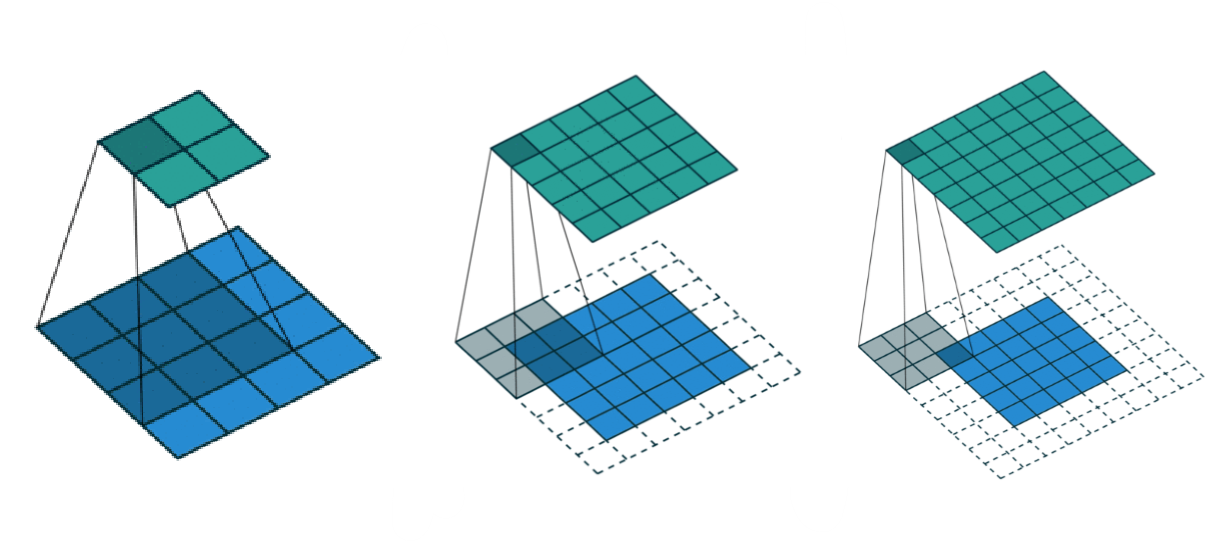
\includegraphics[width=0.7\linewidth]{graphics/padding_cnn.png}
    \caption{Special padding cases for a 2D convolution: to the left valid convolution (no padding), in the middle same convolution (input and output dimensions are the equal), and to the right full convolution (maximum padding).}
    \label{fig:padding-cnn}
\end{figure}

\subsection{Receptive Field}

The \emph{receptive field} of a neuron in a convolutional neural network (CNN) is the region of the input that influences that neuron's output. As you progress deeper into the network, the receptive field generally increases, allowing the network to capture larger context. Understanding the receptive field is essential because it helps you design architectures that capture enough context from the input.
% TODO add image of that

In simpler terms, it is the size of the patch in the input image that contributes to a particular feature in a deeper layer. For layer \(i\) with kernel \(k_i\) and stride \(s_i\), the receptive field can be computed recursively
\[
r_i = r_{i-1} + (k_i - 1) \times S_{i-1},
\]
where \(S_{i-1} = \prod_{j=1}^{i-1} s_j\) is the effective stride. Also, for the first layer applied directly on the input, the receptive field is simply
\[
r_1 = k_1.
\]

\paragraph{Example}
\begin{itemize}
    \item Layer 1: \(k_1 = 3\), \(s_1 = 1 \Rightarrow r_1 = 3\).
    \item Layer 2: \(k_2 = 3\), \(s_2 = 2 \Rightarrow r_2 = 3 + 2 \times 1 = 5\).
\end{itemize}

\subsection{Backpropagation}
TODO
%TODO Explain the backpropagation process in CNNs..

\subsection{CNN Variants}

\subsubsection{ResNet (Residual Networks)}
Deep networks suffer from the \textit{vanishing gradient problem}, where gradients become too small to update weights effectively. ResNet introduces skip connections, allowing layers to learn residual mappings:
\[
F(x) = H(x) - x
\]
where $H(x)$ is the desired mapping.

This technique enables the training of very deep networks (e.g., ResNet-50, ResNet-152).

There are two type of residual blocks

\paragraph{Basic Block} TODO
\paragraph{Bottleneck Block} TODO

\subsubsection{SENet (Squeeze-and-Excitation Networks)}
SENet introduces a channel-wise attention mechanism.
\begin{enumerate}
    \item \textbf{Squeeze:} Global average pooling condenses spatial information.
    \item \textbf{Excitation:} A small fully connected network learns per-channel weights.
    \item \textbf{Recalibration:} Multiplies channel-wise weights with the input feature map.
\end{enumerate}
This enhances feature representation with minimal computational cost.

\subsubsection{Dilated Convolutions}
Useful when spatial redundancy is high. Expands the receptive field without increasing computational cost.

\subsubsection{EfficientNet}
\textit{TODO: Explanation needed.}

\subsubsection{ConvNeXt}
\textit{TODO: Explanation needed.}

% =============================================================
\section{Recurrent Neural Networks (RNNs)}
\textit{TODO: Explanation needed.}
% TODO: Provide an overview of RNNs and include references (e.g., Colah's blog).
% https://colah.github.io/posts/2014-07-NLP-RNNs-Representations/
% https://colah.github.io/posts/2015-08-Understanding-LSTMs/

% =============================================================
\clearpage\newpage

\section{Transformers}
Transformers are effective for language modeling due to their ability to process data in parallel and capture long-range dependencies through attention.

Here are some key points when fine-tuning this type of model:
\begin{itemize}
    \item The dimension of attention keys is critical.
    \item Larger models generally achieve better performance.
    \item Dropout is beneficial.
    \item Positional encodings (sinusoidal or learned) produce similar results.
\end{itemize}

\subsection{Attention Mechanism}
\textit{TODO: This concept needs a dedicated sub section to clearly explain it}
% TODO: Describe the self-attention mechanism in more details

\subsection{Temperature in Transformers}
Temperature is a scaling factor used to control the probability distribution in the self-attention mechanism and during text generation. It modulates the model’s "confidence" in its predictions by adjusting the sharpness of the distributions. Temperature scales the softmax in both self-attention and text generation:

\paragraph{Self-Attention}
\[
e_{ij} = \frac{Q_i \cdot K_j^T}{T\sqrt{d_k}},
\]
where \(T\) adjusts the sharpness.

\paragraph{Text Generation}
\[
P(y) = \operatorname{softmax}\left(\frac{z}{T}\right).
\]

In other words, the parameter \( T \) influences the attention distribution:
\begin{itemize}
    \item \textbf{Low Temperature (\( T < 1 \))}: Results in a sharper distribution, concentrating more strongly on a few tokens with high scores.
    \item \textbf{High Temperature (\( T > 1 \))}: Produces a more diffuse distribution, allowing broader but less pronounced attention.
\end{itemize}


\subsection{Transformer Variants}
\begin{figure}[h!]
    \centering
    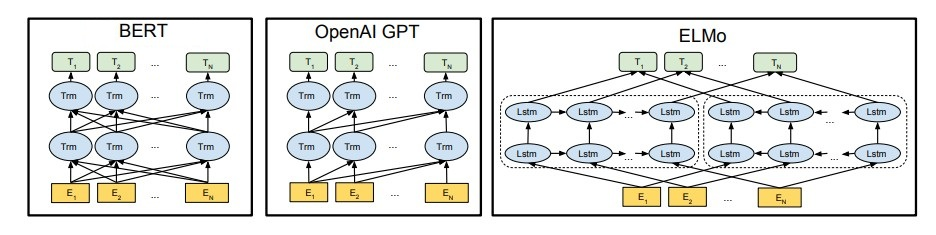
\includegraphics[width=\linewidth]{graphics/transformers_architectures.jpg}
    \caption{Architecture des Transformers. Source : \textit{BERT: Pre-training of Deep Bidirectional Transformers for Language Understanding} (Devlin et al.)}
    \label{fig:transformers_architecture}
\end{figure}

\subsubsection{GPT (Generative Pre-trained Transformer)}
GPT est un modèle basé sur un décodeur Transformer unidirectionnel. Il est entraîné de manière autoregressive pour prédire le token suivant dans une séquence. Son principal atout est la capacité à générer du texte de façon cohérente et fluide.

Les versions plus récentes (GPT-2, GPT-3) utilisent des contextes de taille fixe mais augmentent en taille de modèle pour améliorer la qualité de génération.

\paragraph{GPT3}

Emerging abilities 
- Zero-shot \& Few-shot Prompting
- Scale-up at some point make the performance explode

\subsubsection{BERT (Bidirectional Encoder Representations from Transformers)}
BERT (Bidirectional Encoder Representations from Transformers) is a Transformer-based model introduced by Google AI \cite{devlin2018bert}. It revolutionized NLP by introducing a powerful bidirectional language representation model. It is designed to pre-train deep bidirectional representations by using self-supervised learning, allowing it to achieve state-of-the-art performance on a variety of natural language processing (NLP) tasks.

Ce modele est pré-entraîné à l'aide de la tâche de \textit{Masked Language Modeling} (MLM) ainsi que de la prédiction de la prochaine phrase (NSP).

\paragraph{Masked Language Modeling (MLM)} BERT is pre-trained using a self-supervised learning approach called \textit{Masked Language Modeling} (MLM). In this method:
\begin{itemize}
    \item 15\% of the input tokens are randomly selected for masking.
    \item Of these, 80\% are replaced with a special \texttt{[MASK]} token, 10\% are replaced with a random token, and 10\% remain unchanged.
    \item The model is trained to predict the original tokens based on their surrounding context.
\end{itemize}
This forces BERT to develop a deep bidirectional understanding of text.

\paragraph{Next Sentence Prediction (NSP)} To enhance sentence-level understanding, BERT also uses the \textit{Next Sentence Prediction} (NSP) task:
\begin{itemize}
    \item The model is given two sentences: A and B.
    \item It predicts whether B is the actual next sentence following A or a randomly selected sentence.
\end{itemize}
This task helps BERT learn sentence relationships, which is useful for tasks like question answering and natural language inference.

\paragraph{Fine-tuning}
After pre-training, BERT can be fine-tuned for specific NLP applications by adding task-specific layers on top of the Transformer encoders. Common applications include:
\begin{itemize}
    \item \textbf{Text Classification}: Sentiment analysis, spam detection, topic classification.
    \item \textbf{Named Entity Recognition (NER)}: Identifying people, locations, and organizations in text.
    \item \textbf{Question Answering (QA)}: Extracting answers from passages, such as in the SQuAD dataset.
    \item \textbf{Text Summarization}: Generating concise versions of longer documents.
\end{itemize}

Several improved versions of BERT have been introduced over the years.

\paragraph{RoBERTa} Removes NSP and trains with larger datasets and longer sequences.

\paragraph{ALBERT} Reduces parameter size using factorized embeddings and cross-layer parameter sharing.

\paragraph{DistilBERT} A smaller, faster, and more efficient variant of BERT with fewer layers.

\\

That said, at the moment there isn't much followup on that model as all research are going toward decorder only style architectures like ChatGPT and company. That said, Prof. Aaron mentioned that if he had to bet what is the futur for LLMs in long term, he thinks BERT is because of it's much better performance for same model size.

\subsubsection{ELMo (Embeddings from Language Models)}
ELMo est basé sur des réseaux LSTM bidirectionnels plutôt que sur des Transformers. Il génère des embeddings contextuels pour chaque token en prenant en compte l'ensemble de la phrase. Bien qu'il ait été révolutionnaire pour fournir des représentations riches en contexte, il est moins efficace pour traiter de très longues séquences par rapport aux modèles Transformer modernes.

\subsubsection{Transformer-XL}
Transformer-XL étend le modèle autoregressif en introduisant une récursion au niveau des segments, ce qui permet de réutiliser les états cachés d’un segment à l’autre. Ce mécanisme, associé aux embeddings positionnels relatifs, permet de traiter des contextes beaucoup plus longs que les Transformers standards.

\subsubsection{T5 (Text-to-Text Transfer Transformer)}
T5 adopte une approche encodeur-décodeur en formulant toutes les tâches NLP comme un problème de conversion de texte en texte. Il est particulièrement efficace pour des tâches telles que la traduction, le résumé et la question-réponse. Sa flexibilité en fait un modèle très pertinent dans de nombreux contextes d'applications actuels.

% =============================================================
\clearpage\newpage

\section{Variational Auto-Encoders (VAEs)}
This section introduces the central concepts of Variational Auto-Encoders (VAEs). We discuss how high-dimensional data is modeled using a low-dimensional latent space, derive a tractable variational objective, and present the methods that enable end-to-end learning in these models.

\subsection{Manifold Hypothesis}
In a machine learning context, the manifod hypothesis is the idea that although real world data (like image, audio or text) may exist in a high-dimensional space, the meaningful variations in the data are atually confined to a much lower-dimensional plane or manifold embedded within that high dimensional space. In other words, while each data point is represented by a large number of features, the true degree of freedo (the intrinsic dimensions) are far fewer... There is a limite number of possible values the data points can actually take.

\subsection{Latent Variable Representation}
We represent data \(x\) using latent variables \(z\) via a deterministic mapping:
\[
x = g(z), \quad z \sim \mathcal{N}(0, I)
\]
Here, \(z\) encapsulates the underlying factors of variation, and the decoder \(g\) reconstructs the high-dimensional data from \(z\).

\subsubsection{Maximum Likelihood}
The goal would then be to maximise a mapping such that
\[
\log p(x) = \log \int p(x|z)p(z)\,dz
\]
However, the integral over \(z\) is generally intractable.

\subsection{The Variational Objective}
To bypass the intractability of directly computing \(\log p(x)\), VAEs optimize a approximated lower bound on the log-likelihood.

\subsubsection{ECLL (Expected Complete-Data Log-Likelihood)}
An intermediate formulation approximates the complete-data log-likelihood:
\[
\mathbb{E}_{q(z|x)}[\log p(x,z)]
\]
This expectation serves as a proxy by averaging over the latent variable distribution.

\subsubsection{KL Divergence}
The KL divergence measures the difference between the approximate posterior and the prior:
\[
D_{\text{KL}}(q(z|x) \Vert p(z|x)) = -\int q(z|x)\,\log \frac{q(z|x)}{p(z|x)} \,dz
\]
This term regularizes the latent space, ensuring that \(q(z|x)\) remains close to the simple prior \(p(z|x)\).

\subsubsection{ELBO}
The Evidence Lower Bound (ELBO) is defined as:
\[
\text{ELBO} = \mathbb{E}_{q(z|x)}[\log p(x|z)] - D_{\text{KL}}(q(z|x) \Vert p(z))
\]
Maximizing the ELBO leads to a practical training objective that both reconstructs \(x\) and regularizes \(q(z|x)\).

\subsection{Backpropagation}
The entire VAE, including both encoder and decoder, is trained end-to-end via backpropagation using gradients derived from the variational objective.

\subsubsection{The Reparameterization Trick}
To enable gradient flow through sampling, we reparameterize \(z\) as:
\[
z = \mu(x) + \sigma(x)\epsilon, \quad \epsilon \sim \mathcal{N}(0, I)
\]
This neat transformation allows us to treat the random sampling as a differentiable operation.

\subsection{VAE Variants}

\subsubsection{VAE-IAF}
To achieve a richer posterior, we apply a series of invertible transformations:
\[
z_T = f_T \circ \cdots \circ f_1(z_0)
\]
Inverse Autoregressive Flow (IAF) enables the approximate posterior to capture complex dependencies.

\subsubsection{IWAE (Weighted Importances)}
An improved variational bound is obtained by importance weighting:
\[
\log p(x) \approx \log \frac{1}{K} \sum_{k=1}^{K} \frac{p(x,z_k)}{q(z_k|x)}
\]
Multiple samples tighten the bound and enhance the model's performance.

\subsubsection{SVG / VRNN }
For sequential data, stochastic variational recurrent networks incorporate latent variables into recurrent architectures. This approach, known as SVG or VRNN, models temporal dependencies alongside latent representations.

% =============================================================
\clearpage\newpage

\section{Diffusion models}

% TODO This section needs lots of love and improvements. (I need to summarize my notes and clean them up!)

One interesting note in the course was diffusion models as spectral noise. You saw in that plot that when you do the process of adding the gaussian noise to the image, you loose the high frequency information of the image and you just keep the low frequency information.

The difference of the model diffusion and VAE is that VAE takes from the latent space in one shot but the diffusion models go from noisy to no noise iteratively. This gives time to the model to correct himself, one of the reason why the diffusion models are so performing at the moment.

\subsection{Controlling Diffusion models (Part 2)}

Il y at un tradeoff entre la quality et la quantite des images generer

Tu plug un encoder text avant par exemple stable diffusion alors les deux captions
"An image of a loaf of bread in the shape of a cat."
"An image of a cat in the shape of a loaf of bread"

You get almost the same thing which is because the word encoder mix them up and cause the caption to loose the nuances.

Difficulte avec la spacialite dans la generation des images. Genre quelque chose a gauche et un autre a droite.

Aussi difficulte dans les interactions entre les objets et choses.

Dalle essaye toujours de toujours generer 10:10 dans les montres. C'est un biais pcq les photos de montre sur le net c'est tres tres souvent 10:10.

Diffusion discret sont le future?? Mais pas encore de resultats empirique

Les modele de diffusion discret opperere sur les nombres reel??

Toujours chain de markov

% =============================================================
\clearpage\newpage

\section{Reinforcement Learning}
% TODO: Add notes and video references on reinforcement learning.

\subsection{Reward Hacking}

\subsection{Markov Decision Process}

\subsection{Policies}

\subsection{Bellman Equations}

\subsection{Value-Based RL}

\subsubsection{Goal} Learn value functions

\subsubsection{Policy} You derive the policy from the value function, typically by choosing the action with the highest value (greedy policy).

\subsubsection{Q-Learning}

\subsubsection{Deep Q-Learning}

\subsection{Policy-Based RL}

\subsubsection{Goal} Learn policy parameters

\subsubsection{Policy} You directly learn a parameterized policy (e.g., neural network) that outputs actions or action probabilities.

\subsection{Actor-Critic}

\subsubsection{Policy} You learn both a policy (the actor) and a value function (the critic). The actor selects actions, while the critic evaluates them.

% =============================================================
\clearpage\newpage

\section{Reinforcement Learning from Human Feedback (RLHF)}

Language models are not aligned with user intent [Ouyang et al., 2022]. Finetuning can help!

There are two steps to this situation.

First step is pretraining on language modeling (lots of text; learn general things!)

Second step is fietuning with human feedback (many tasks, many labels, adapt to the tasks!)

We can generally do two type of finetuning. One is supervised training and the other by reinforcement (RLHF).

\subsection{Flan-T5}

\subsection{Limitations of Finetuning}

One problem is that we have open-ended questions that are difficult to evaluate what is "good" and what is "bad". Especially in creative tasks. If we finetune too much on those tasks there will be overfitting quickly.

Another problem is that language modeling penalizes all token-level mistakes equally, but some errors are worse than others.

For exemple when you evaluate the output of the model, we will use cross-entropy based on the probabilities output of the model. Why it doesn't punish the model too much even if he output a synonym is that in the probabilities, the synonimes will generally both at the same \%. Therefor the model is not too much punished.

\subsection{Human-in-the-loop}

This method is by far the best way to finetune models but there are some big problems with this technique too.

One of the main problem is that this process is expensive. The solution that companies have been using is to model their preferences as a separate (NLP) problem. [Knox and Stone, 2009]
- One exemple is chatgpt options to thumbs up/down the awnsers, regenerate awnsers and make the user choose between two awnsers.

Another problem is that human judgment is noisy and misscalibrated. A solution that was found was that instead of asking for direct ratings, the system should ask for pairwise comparisons, which can be more reliable. [Phelps et al., 2015; Clark et al., 2018]

\subsection{Reward }
Almost always this for RLHF

\subsection{InstructGPT}
Step 1 (Supervised training): Collect demonstration data and train a supervised policy.
Step 2... 
Step 3...

\subsection{LLM-as-a-judge}

- PAS UTILISER POUR REINFORCEMENT!! JUST BENCHMARKING

Instead of using a human in the feed-back-loop, we can use a LLM to judge the awnsers. This method has been increasing in popularity in recent years. We generally choose the biggest model to make the judgments on the awnsers.

Here are some notes on that:
- Models are heavily positionally biased
- Models often rate on syntax & response length

\subsection{Benchmarks and comparisons}

\subsubsection{MT Bench}

% ============================================================
\clearpage\newpage

\section{Self-Supervised Learning}

The main idea behind self-supervision is to design auxiliary (“pretext”) tasks that generate supervisory signals directly from the structure of the data, thus eliminating the need for manual labels. These pretext tasks force the model to learn meaningful representations that are useful when transferred to downstream tasks.

\subsection{Pretext Task Paradigm}

At its core, the self-supervised framework leverages pretext tasks to generate supervisory signals from the data itself.

\begin{itemize}
    \item \textbf{Data Transformation:} Raw inputs (e.g., images) are modified using operations such as cropping, permutation, or geometric transformation.
    \item \textbf{Task Definition:} The network is trained to predict the transformation, the relative context, or to compare different views of the same instance.
    \item \textbf{Representation Learning:} In solving the pretext task, the network learns high-level semantic or structural features that generalize well.
\end{itemize}

\subsection{Spatial Context and Structural Tasks}
\subsubsection{Context Prediction}
\begin{itemize}
    \item \textbf{Task:} Given two patches from the same image (with a spatial gap and random jitter), the network predicts their relative spatial configuration.
    \item \textbf{Architecture:} Utilizes a \emph{Siamese network} structure with shared weights to process each patch, and a late-fusion module that combines features (often from a fully connected layer) for classification into one of several spatial configurations.
    \item \textbf{Design Consideration:} Incorporates mechanisms such as patch gaps, jitter, and color preprocessing to prevent the network from learning trivial (low-level) solutions.
\end{itemize}

\subsubsection{Jigsaw Puzzles}
\begin{itemize}
    \item \textbf{Task:} An image is split into tiles (e.g., a 3$\times$3 grid) and then randomly permuted. The network is tasked with reassembling the puzzle.
    \item \textbf{Architecture:} Implements a multi-stream network where each tile is processed by a branch with tied weights, followed by a permutation classification layer that predicts the correct arrangement from a carefully chosen set of possibilities.
    \item \textbf{Outcome:} This method forces the model to understand both object parts and the overall structure.
\end{itemize}

\subsubsection{Rotation Prediction}
\begin{itemize}
    \item \textbf{Task:} The network must predict the rotation applied to an image (typically one of 0°, 90°, 180°, or 270°).
    \item \textbf{Architecture:} Consists of a single-stream CNN that extracts features from the rotated image, feeding into a classification head that outputs a probability distribution over rotations.
    \item \textbf{Intuition:} The task compels the network to understand the configuration of objects, as accurate rotation prediction requires awareness of object semantics.
\end{itemize}

\subsection{Contrastive Learning and Beyond}

Contrastive methods and their extensions drive learning by comparing different views of the same instance against other samples, enforcing invariance across augmentations.

\subsubsection{MoCo (Momentum Contrast)}
\begin{itemize}
    \item \textbf{Idea:} Build a dynamic dictionary using a large queue of negative examples and a momentum-updated encoder.
    \item \textbf{Architecture:} 
    \begin{itemize}
        \item Dual encoders: a query encoder for the current mini-batch and a key encoder updated via a momentum mechanism.
        \item A contrastive loss (e.g., InfoNCE) that encourages the query representation to align with its positive key while differentiating from negatives stored in the queue.
    \end{itemize}
    \item \textbf{Advantage:} Decouples the dictionary size from the mini-batch size while ensuring stable key representations.
\end{itemize}

\subsubsection{SimCLR (Simple Framework for Contrastive Learning)}
\begin{itemize}
    \item \textbf{Idea:} Leverage strong data augmentations to create varied views of the same image and pull their representations together.
    \item \textbf{Architecture:} A standard CNN backbone is augmented with a projection head and trained with a contrastive loss very similar to InfoNCE using large batch sizes and temperature scaling.
    \item \textbf{Outcome:} Establishes a simplified yet highly competitive baseline in self-supervised learning.
\end{itemize}

\subsubsection{CLIP (Contrastive Language–Image Pre-training)}
\begin{itemize}
    \item \textbf{Idea:} Align image representations with natural language descriptions using a bi-encoder architecture.
    \item \textbf{Architecture:} Includes an image encoder and a separate text encoder. A contrastive loss is used to maximize the similarity of matching image--text pairs and minimize it for non-matching pairs.
    \item \textbf{Impact:} Enables learning of rich, multi-modal representations that transfer effectively across vision and language tasks.
\end{itemize}

\subsubsection{BYOL (Bootstrap Your Own Latent)}
\begin{itemize}
    \item \textbf{Idea:} Achieves self-supervised learning without explicit negative examples by maintaining an online and a target network.
    \item \textbf{Architecture:} Both networks (often with an added projection head) process augmented views of the same image. The target network is updated as a moving average of the online network.
    \item \textbf{Outcome:} Yields robust representations through careful design and momentum updates despite the absence of negative pairs.
\end{itemize}

\subsubsection{Barlow Twins}
\begin{itemize}
    \item \textbf{Idea:} Reduce redundancy in feature dimensions by pushing the cross-correlation matrix between different augmentations toward the identity matrix.
    \item \textbf{Architecture:} Uses a shared backbone with a projection head for two augmented views. The loss function combines terms for invariance and decorrelation.
    \item \textbf{Advantage:} Avoids the need for explicit negative sampling while still enforcing meaningful representation learning.
\end{itemize}

\subsubsection{DINO (Self-Distillation with No Labels)}
\begin{itemize}
    \item \textbf{Idea:} Employ a teacher--student framework, where the teacher (an exponential moving average of the student) provides soft targets that stabilize training.
    \item \textbf{Architecture:} Both the student and teacher networks process multiple augmented views, and a distillation loss aligns the student’s outputs with the teacher’s.
    \item \textbf{Outcome:} Generates strong clustering and attention maps, leading to highly transferable features.
\end{itemize}

\subsubsection{JEPA (Joint Embedding Predictive Architecture) and I-JEPA (Improved JEPA)}
\begin{itemize}
    \item \textbf{Idea:} Go beyond simple instance discrimination by predicting the representation of one part of an image from its surrounding context.
    \item \textbf{Architecture:} Consists of a context encoder and a predictor network that work on partially observed images (or masked regions) to predict the representations for missing parts.
    \item \textbf{Enhancements in I-JEPA:} Refinements in both prediction and embedding strategies yield more robust and transferable features.
    \item \textbf{Significance:} Aligns with modern trends emphasizing joint embedding frameworks without the explicit need for negative sampling.
\end{itemize}

\subsection{Knowledge Distillation}

\textbf{Knowledge Distillation} has traditionally been used to transfer information from a “teacher” model to a “student” model in supervised settings. It allows further refinements by predicting content based on context and transferring rich teacher knowledge to student models.

Methods like DINO utilize a teacher--student formulation in a label-free setting, where the student is trained to mimic the softened outputs of the teacher.

This process generally enhances feature robustness and improves transferability by internalizing richer representations.

\end{document}